\documentclass[12pt]{article}
\usepackage[utf8]{inputenc}
\usepackage{graphicx}
\usepackage[labelfont=bf,label]{caption}
\title{essay}
\author{Shriram Angadrao Fajage}
\date{August 2020}

\begin{document}

\maketitle

\section{Introduction}
India is the second most populated country in the world with nearly a fifth of the world's population. According to the 2019 revision of the World Population Prospects[6][7] population stood at 1,352,642,280.

During 1975–2010, the population doubled to 1.2 billion. The Indian population reached the billion mark in 1998. India is projected to be the world's most populous country by 2024,[8] surpassing the population of China. It is expected to become the first country to be home to more than 1.5 billion people by 2030, and its population is set to reach 1.7 billion by 2050.[9][10] Its population growth rate is 1.13 percent, ranking 112th in the world in 2017.[11]

India has more than 50 percent of its population below the age of 25 and more than 65 percent below the age of 35. It is expected that, in 2020, the average age of an Indian will be 29 years, compared to 37 for China and 48 for Japan; and, by 2030, India's dependency ratio should be just over 0.4.[12]. However, the number of children in India peaked more than a decade ago and is now falling. The number of children under the age of five (under-5s) peaked in 2007; since then the number has been falling. The number of Indians under 15 years old peaked slightly later (in 2011) and is now also declining. [13]

India has more than two thousand ethnic groups,[14] and every major religion is represented, as are four major families of languages (Indo-European, Dravidian, Austroasiatic and Sino-Tibetan languages) as well as two language isolates (the Nihali language[15] spoken in parts of Maharashtra and the Burushaski language spoken in parts of Jammu and Kashmir (Kashmir)). 1,000,000 people in India are Anglo-Indians and 700,000 Westerners from the United States are living in India.[16] They represent over 0.1% of the total population of India.

Further complexity is lent by the great variation that occurs across this population on social parameters such as income and education. Only the continent of Africa exceeds the linguistic, genetic and cultural diversity of the nation of India.[17]

The sex ratio is 944 females for 1000 males (2016) (940 per 1000 in 2011[18]). This ratio has been showing an upwards trend for the last two decades after a continuous decline in the last century.[19]
\subsection{analysis}
\begin{figure}
    \centering
    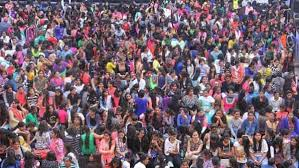
\includegraphics[width=1.2\linewidth]{population}
    \caption{population}
    
\end{figure}

\begin{tabular}{|c|c|}
    \hline
    census year & population \\ \hline
    1951 & 361088000 \\ \hline
    1961 & 439235000 \\ \hline
    1971 & 548160000 \\ \hline
    1981 & 683329000 \\ \hline
    1991 & 846387888 \\ \hline
    2001 & 1028737436 \\ \hline
    2011 & 1210726932 \\ \hline
\end{tabular}

\end{document}
